% !TeX root = main.tex

\chapter{Long Short Term Memory}

Objectif principal de ce projet, l'architecture neuronale Long Short Term Memory
(LSTM) est décrite dans cette partie. Tout comme les autres architectures
neuronales, elle est constituée d'un assemblage de blocs élémentaires qui
disposent d'un ensemble de variables, appelés poids, à adapter lors de la phase
d'apprentissage afin de reproduire une fonction. Cependant, la cellule
élémentaire d'un réseau LSTM est bien plus complexe que celle d'un réseau
neuronal à perceptrons.

\medskip

La dénomination LSTM vient du fait que ce type de réseau possède une mémoire de
plus longue durée que des structures plus simples avec une seule couche de
neurones. Ainsi, il sera possible d'apprendre des fonctions telles que la
grammaire de Reber double, ou bien de générer du texte après avoir appris des
écrits de Shakespeare.

\medskip

LSTM est notamment utilisé dans des applications de reconnaissance vocale.

\medskip

\section{Théorie}
\subsection{Cellule LSTM}

La cellule LSTM est constituée de différents réseaux de perceptrons.
La principale différence avec un simple réseau à perceptrons est que la cellule
possède une mémoire. Il s'agit d'un vecteur qui sera pris en entrée (en même
temps que l'entrée au temps $t$ et la sortie du temps $t-1$, modifié par
les entrées au temps $t$ et renvoyé au temps $t+1$ dans la même cellule.

\medskip

Chaque réseau de perceptrons représente une opération sur la mémoire, tous
prennent en entrée l'entrée de la cellule au temps $t$ et sa sortie au temps
$t-1$:

\begin{itemize}
  \item La "input gate" est le réseau qui effectue des opérations d'addition
    sur la mémoire.
  \item La "block input" est le réseau qui définit les coordonnées de la mémoire
    qui seront affectées par l'input gate.
  \item La "forget gate" est le réseau qui détermine quelles coordonnées de la
    précédente mémoire garder à $t$. Ce réseau n'est pas présent dans toutes les
    implémentations, on pourra étudier l'impact de sa présence.
  \item La "output gate" est le réseau qui détermine les sorties de la cellule.
\end{itemize}

\begin{figure}[!ht]
\begin{center}
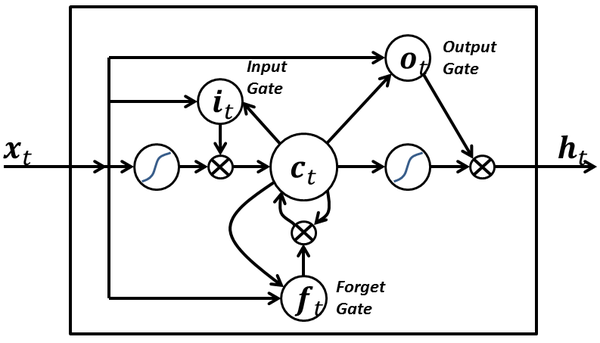
\includegraphics[width=0.6\linewidth]{images/lstm.png}
\end{center}
\caption{Cellule LSTM}
% TODO : Credits or new figure
\end{figure}

\subsection{Propagation}

Soit N la taille du vecteur de sortie et M la taille du vecteur d'entrée, on
peut définir les matrices de poids :

\begin{itemize}
  \item Poids relatifs à l'entrée : $W_z$, $W_i$, $W_f$,
    $W_o \in \mathbb{R}^{M \times N}$
  \item Poids relatifs à la sortie précédente : $R_z$, $R_i$, $R_f$,
    $R_o \in \mathbb{R}^{N \times N}$
  \item Poids des biais : $b_z$, $b_i$, $b_f$,
    $b_o \in \mathbb{R}^N$
\end{itemize}

Soit $\sigma$ la fonction d'activation sigmoide $\sigma(x)=\frac{1}{1+e^{-x}}$,
$x^t$ l'entrée au temps $t$, $y^t$ la sortie de la cellule au temps $t$, $c^t$
la mémoire de la cellule au temps $t$ et $\odot$ le produit d'Hadamard,
on peut définir les expressions suivantes pour les sorties de chaque couche de
perceptrons :

\medskip

\begin{itemize}
  \item block input :
    $$\overline{z}^t = W_z x^t + R_z y^{t-1} + b_z$$
    $$z^t = \tanh(\overline{z}^t)$$
  \item input gate :
    $$\overline{i}^t = W_i x^t + R_i y^{t-1} + b_i$$
    $$i^t = \sigma(\overline{i}^t)$$
  \item forget gate :
    $$\overline{f}^t = W_f x^t + R_f y^{t-1} + b_f$$
    $$f^t = \sigma(\overline{f}^t)$$
  \item output gate :
    $$\overline{o}^t = W_o x^t + R_o y^{t-1} + b_o$$
    $$o^t = \sigma(\overline{o}^t)$$
\end{itemize}


\subsection{Algorithmes d'apprentissage}
L'algorithme d'apprentissage est un algorithme BPTT appliqué aux cellules
LSTM considérées.

\begin{figure}[!ht]
\begin{center}
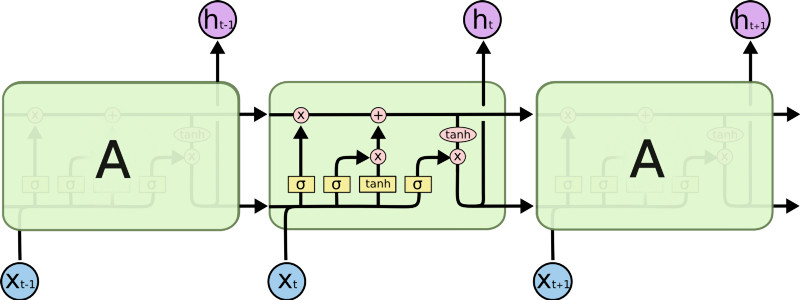
\includegraphics[width=0.8\textwidth]{images/lstm-bptt.png}
\end{center}
\caption{Dépliement du temps dans l'espace style BPTT}
% TODO : Credits or new figure
\end{figure}

\section{Implémentation}

L'implémenation est effectuée en C++ via la librairie de calcul matriciel
Eigen3. Toutes les matrices sont des objets de type Eigen::MatrixXd (matrice de
double) et les vecteurs des objets de type Eigen::VectorXd.

\medskip

L'aléatoire utilisé est celui natif en C et C++ : rand.
La génération de la graine se fait à partir du temps à la milliseconde pour
éviter une initialisation déterministe dans le cas de l'execution de plusieurs
runs consécutifs. Pour cela la librairie 'sys/time.h' est utilisée, avec un
appel propre aux systèmes UNIX.

\bigskip

\subsection{Structure de données}

Le code se décompose en plusieurs éléments :

\medskip

\begin{itemize}

  \item Les poids LSTM
  \item La cellule LSTM
  \item Le réseau LSTM

\end{itemize}
\subsubsection{Les poids LSTM}

La classe poids regroupe toutes les matrices de poids des différents noeuds
de la cellule LSTM. Ces dernier sont : input\_gate, input\_block, output\_gate.
Pour chacun des noeuds il existe deux matrices de poids : une relative à
la sortie précédente de la cellule, et l'autre relative à l'entrée de la
cellule. Enfin, il existe aussi pour chaque noeud un vecteur de biais.

\medskip

Tous ces éléments sont amenés à être modifiés, c'est pourquoi l'on crée pour
chacun une matrice (ou un vecteur) de delta : modifications à appliquer.

\medskip

Enfin, les méthodes de l'objet poids LSTM sont le constructeur et
l'application des variations de poids (qui remet par la même occasion à 0
les delta-poids).

\subsubsection{La cellule LSTM}

La cellule LSTM est l'objet élémentaire du réseau. Elle est créée en prenant
pour arguments un pointeur vers un objet de type poids, et les informations de
dimentions d'entrée et sortie.

\medskip

Elle dispose des méthodes nécessaires à la propagation et la rétropropagation
à travers une cellule LSTM.
Pour renvoyer plusieurs vecteurs (la sortie, la mémoire) on utilise ici des
std::vector<Eigen::VectorXd> dont chaque case correspond à un vecteur que l'on
souhaite renvoyer.

\medskip

La propagation n'est rien d'autre qu'une application directe des formules de la
propagation à travers une cellule LSTM. Sont stockées certaines valeurs
intermédiaires pertinentes pour éviter leur calcul à nouveau lors de la
rétropropagation.

\medskip

Lors de la rétropropagation, les variations de poids sont calculées et ajoutées
aux attributs delta\_poids de l'objet weightsLSTM. La fonction de cout choisie
est la fonction de coût quadratique (divisée par deux), sa dérivée étant alors
la différence entre sortie obtenue et sortie attendue.

\bigskip

Les attributs sont donc les suivants :

\begin{itemize}
  \item \verb+WeightsLSTM* weights+ l'objet poids qui sera utilisé par la
    cellule pour calculer les sorties de chaque noeud ;
  \item \verb+Eigen::VectorXd input+ vecteur des entrées de la cellule à
    l'instant $t$ ;
  \item \verb+Eigen::VectorXd previous\_output+ vecteur des sorties de la
    cellule à l'instant $t-1$ ;
  \item \verb+Eigen::VectorXd previous\_cell\_state+ mémoire de la cellule
    à l'instant $t-1$ ;
  \item \verb+Eigen::VectorXd input\_gate\_out+ sortie du noeud input\_gate
    à l'instant $t$ ;
  \item \verb+Eigen::VectorXd input\_block\_out+ sortie du noeud input\_block
    à l'instant $t$ ;
  \item \verb+Eigen::VectorXd output\_gate\_out+ sortie du noeud output\_gate
    à l'instant $t$ ;
  \item \verb+Eigen::VectorXd cell\_state+ mémoire de la cellule à
    l'instant $t$ ;
  \item \verb+Eigen::VectorXd cell\_out+ sortie de la cellule à l'instant $t$.
\end{itemize}

Les méthodes sont donc les suivantes :

\begin{itemize}
  \item \verb+compute( Eigen::VectorXd previous\_output,
    Eigen::VectorXd previous\_memory, Eigen::VectorXd input)+ la methode qui
    calcule la sortie de chaque noeud de la cellule, puis la sortie de la
    cellule. Renvoie \verb+<cell\_out, cell\_state>+ ;
  \item \verb+compute\_gradient(
    Eigen::VectorXd deltas, Eigen::VectorXd previous\_delta\_cell\_in,
    Eigen::VectorXd previous\_delta\_cell\_state)+ la methode qui calcule le
    gradient en entrée de la cellule en fonction des gradients en sortie.
    Renvoie \verb+<delta\_input, delta\_cell\_state>+.
\end{itemize}

\subsubsection{Le réseau LSTM}

Le réseau LSTM est principalement constitué d'un std::vector<CellLSTM>.
A chaque temps $t$, une nouvelle cellule est crée et stockée à l'index i du
vector.

\medskip

La propagation s'effectue cellule par cellule, chaque cellule prenant en entrée
la sortie de la précédente à $t-1$ ainsi que l'entrée du réseau au temps
$t$. De même, la rétropropagation s'effectue de la dernière cellule du vector à
la première.

\bigskip

Les attributs sont donc les suivants :

\begin{itemize}
  \item
  \item \verb+WeightsLSTM* weights+ l'objet poids utilisé pour la création de
    chaque cellule;
  \item \verb+int input\_size+ la taille de l'entrée;
  \item \verb+int output\_size+ la taille de la sortie ;
  \item \verb+int layer\_size+ la taille des couches cachées ;
  \item \verb+std::vector<Cell> cells+ le vecteur dans lequel sont stockées les
    cellules crées pour chaque instant $t$ de la propagation.
\end{itemize}

\bigskip

Les méthodes sont donc les suivantes :

\begin{itemize}
  \item \verb+propagate(std::vector<Eigen::VectorXd> inputs)+ crée à chaque
    instant $t$ une nouvelle cellule et utilise sa methode \verb+compute+
    pour calculer l'entrée de la suivante ;
  \item \verb+backpropagate(std::vector<Eigen::VectorXd> expected\_outputs)+
    rétropropage le gradient de la dernière cellule à la première en utilisant
    la methode \verb+compute\_gradient+ de chaque cellule;
\end{itemize}

\section{Résultats}
Ci-dessous des représentations de l'apprentissage au cours du temps du réseau sur des
grammaires de Reber, simple et double. \\
En abscisse, le nombre de mots appris, en ordonnée le taux de réussite, testé à
intervalles réguliers sur un échantillon de données de test choisies aléatoirement
dans l'ensemble de test. \\
La zone grise correspond à l'intervalle de confiance à $95\%$ sur le nombre d'exécutions
précisé.\\
Le réseau utilisé est composé d'une couche de 30 cellules LSTM, avec un learning
rate de $0.1$.

\subsection{Grammaire de Reber simple}
Pour une grammaire de Reber simple, la réussite est déterminée par la prédiction
correcte de toutes les transitions des mots testés.

\begin{figure}[!ht]
\begin{center}
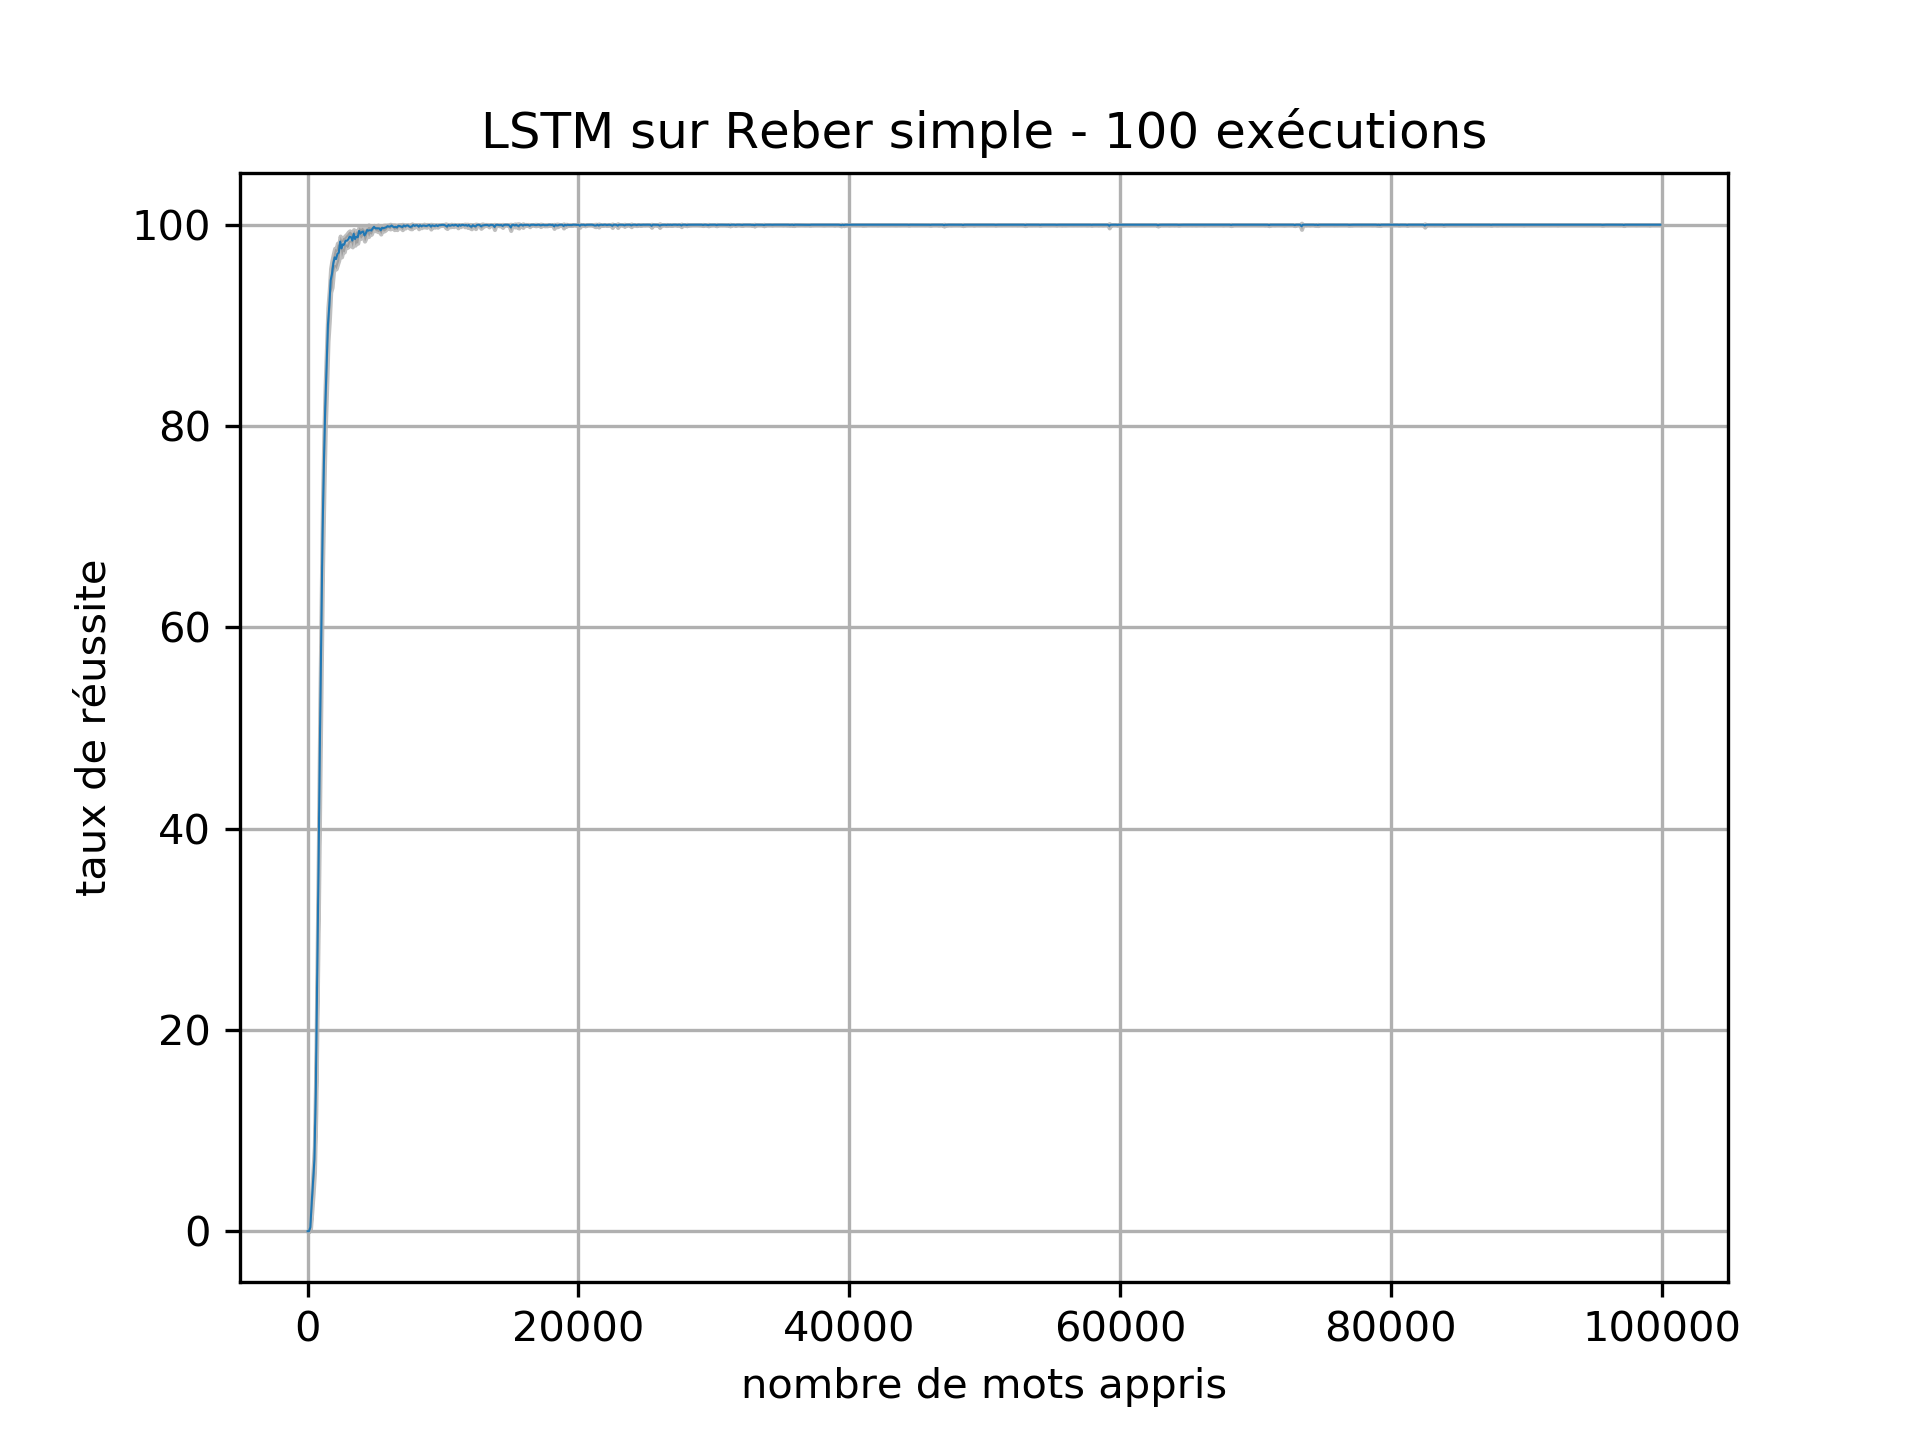
\includegraphics[width=0.8\textwidth]{images/results/lstm_simplereber_ls30_lr01.png}
\caption{Apprentissage au cours du temps, LSTM sur grammaire de Reber simple}
\end{center}
\end{figure}

\subsection{Grammaire de Reber symétrique}
Pour une grammaire de Reber symétrique, réussite est déterminée par la prédiction
correcte de la première et la dernière transition des mots testés.

\begin{figure}[!ht]
\begin{center}
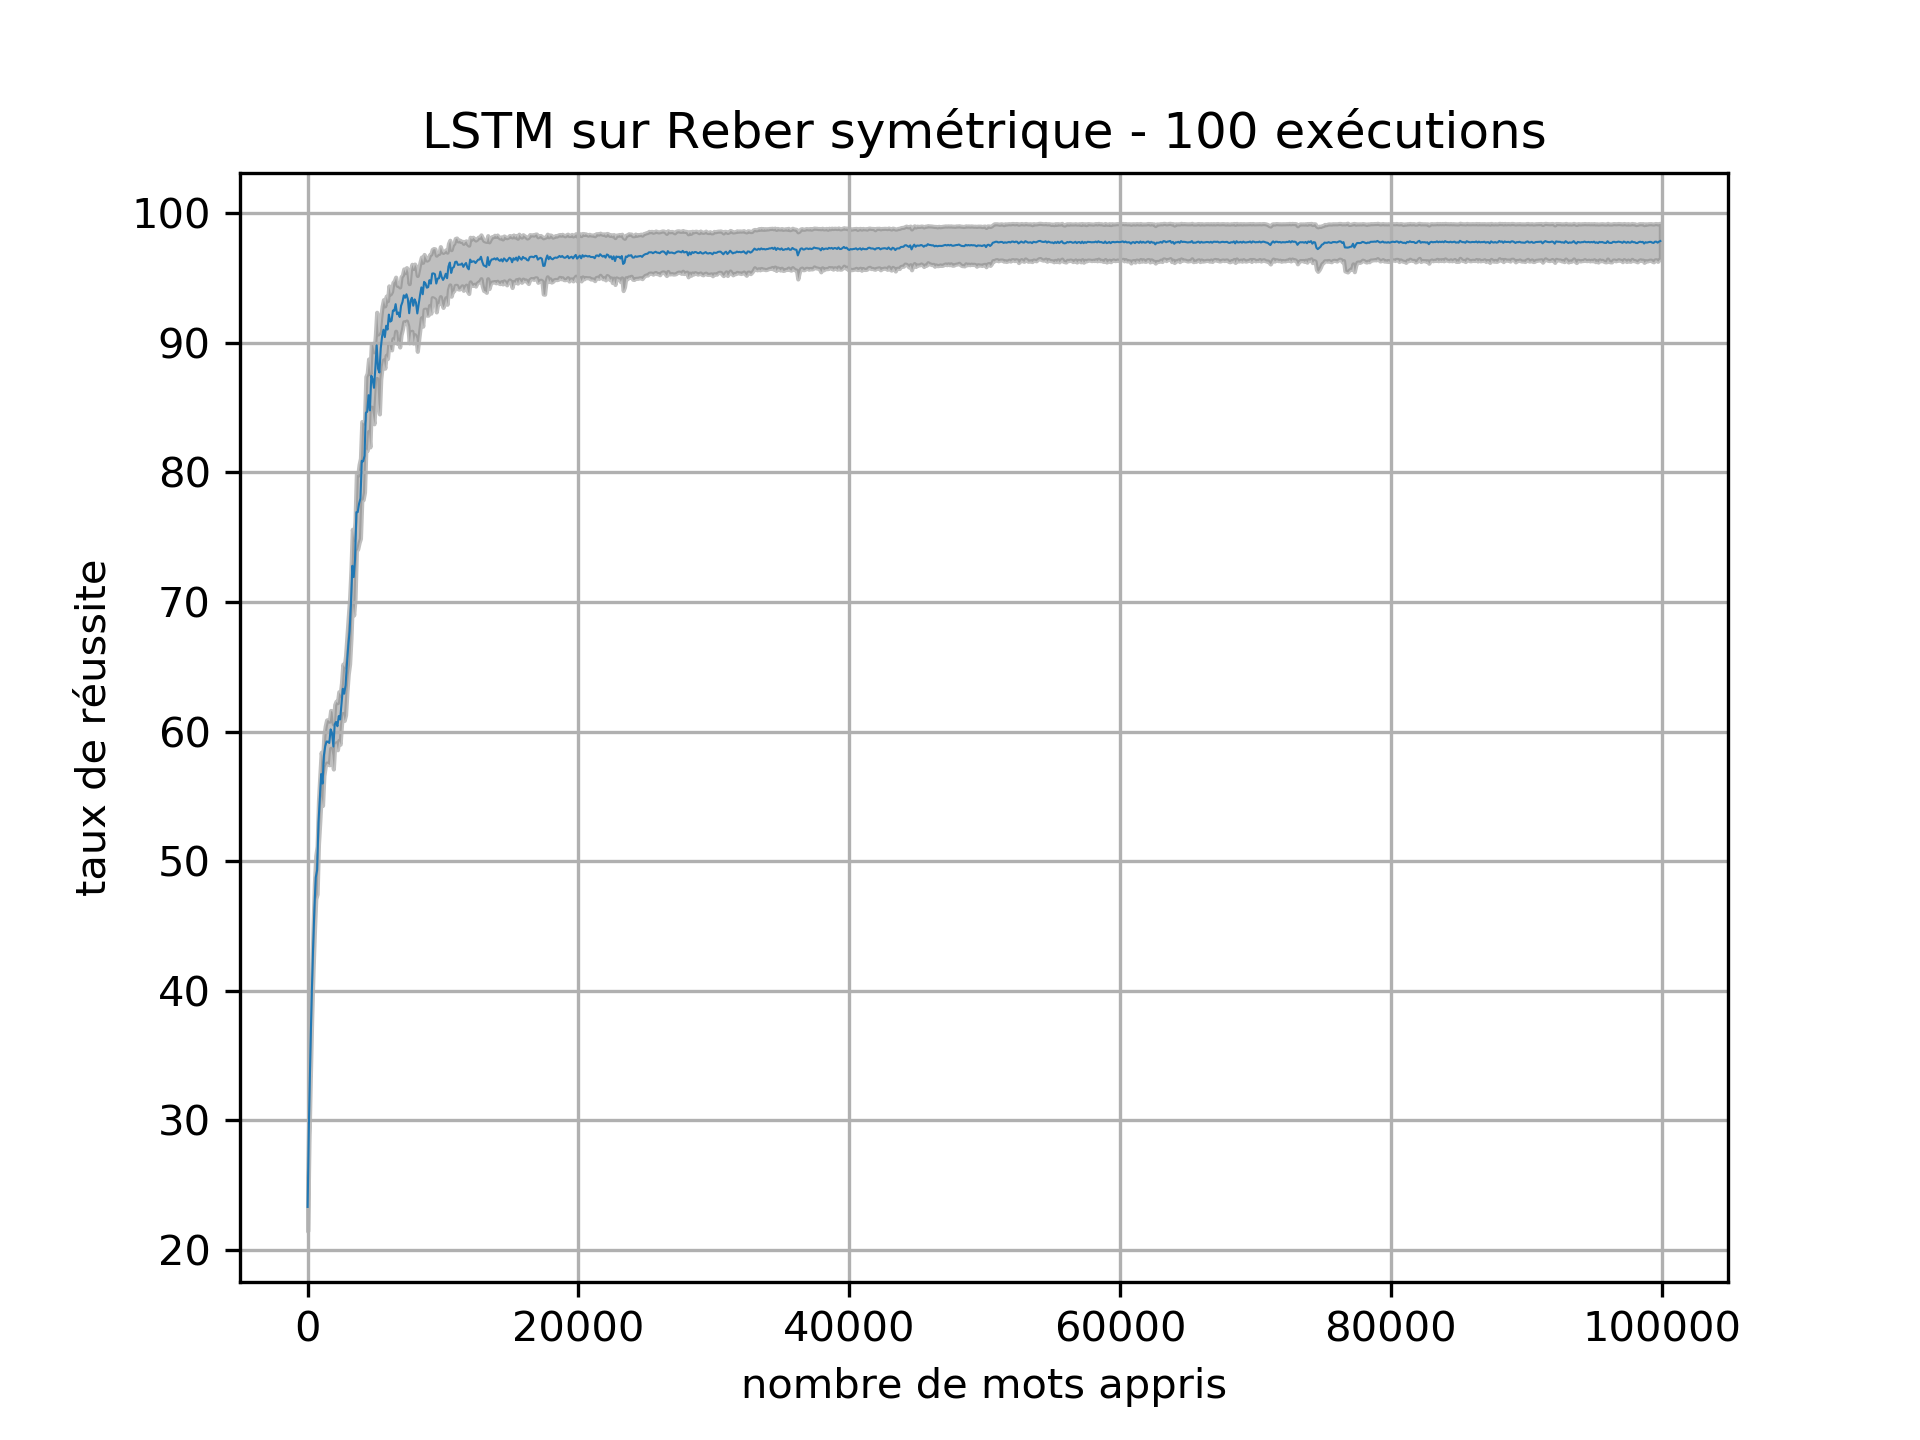
\includegraphics[width=0.8\textwidth]{images/results/lstm_doublereber_ls30_lr01.png}
\caption{Apprentissage au cours du temps, LSTM sur grammaire de Reber symétrique}
\end{center}
\end{figure}
